\chapter{Suporte Tecnológico}

Afim de manter e disponibilizar o código e os artefatos gerados a partir deste trabalho, bem como o ambiente utilizado para a construção do framework, serão apresentadas as principais ferramentas candidatas a serem utilizadas durante o seu desenvolvimento.

\section{Ferramentas de Desenvolvimento}

\subsection{Git}

O Git\footnote{\url{https://git-scm.com/}} é um sistema de controle de versão distribuído, projetado basicamente para facilitar a vida de quem quer executar projetos em equipe de forma segura. Foi criado por Linus Torvalds, pois precisava de um controle de versão rápido e que pudesse lidar com uma grande atividade envolvida no desenvolvimento do Kernel do Linux. Linus, desejava um ferramenta livre, não encontrando, ele decidiu criar o Git. Ele foi batizado em referência ao próprio Linus, no inglês britânico, Git é uma gíria para ``cabeça-dura''.

Uma vantagem do Git é a possibilidade de controlar o projeto de forma descentralizada, ou seja, sem a exigência de um servidor mestre. E cada arquivo rastreado pelo Git tem seu conteúdo verificado usando o algoritmo de criptografia SHA-1.

O que faz o Git funcionar mesmo é sua habilidade de detectar mudanças em arquivos, não só que uma mudança ocorreu, mas também onde mudança aconteceu. Podendo desfazer as alterações que estão com problemas, voltando para a versão mais estável.

\begin{figure}[!h]
	\centering
	
\includegraphics[scale=0.35]{figuras/capitulo3/git.eps}
	\caption{Logo do Git}
	\label{git}
\end{figure}

\subsection{GitHub}

O GitHub\footnote{\url{https://github.com}}, lançado 2008 e feito em Ruby on Rails, provê um armazenamento em nuvem (\textit{Cloud}), onde se pode hospedar projetos utilizando o Git como controle de versão. O GitHub possui funcionalidades de um rede social como \textit{feeds}, \textit{followers}, wiki e gráficos para apresentar como os desenvolvedores trabalham em um repositório. Este lado social é interessante para descobrir novos projetos e receber ajuda em projetos particulares. É importante ressaltar que o repositório fornecido pelo GitHub é gratuito. Entretanto, este repositório fica como de acesso público, porém, existem planos comerciais no qual o repositório pode se tornar privado.

\begin{figure}[!h]
	\centering
	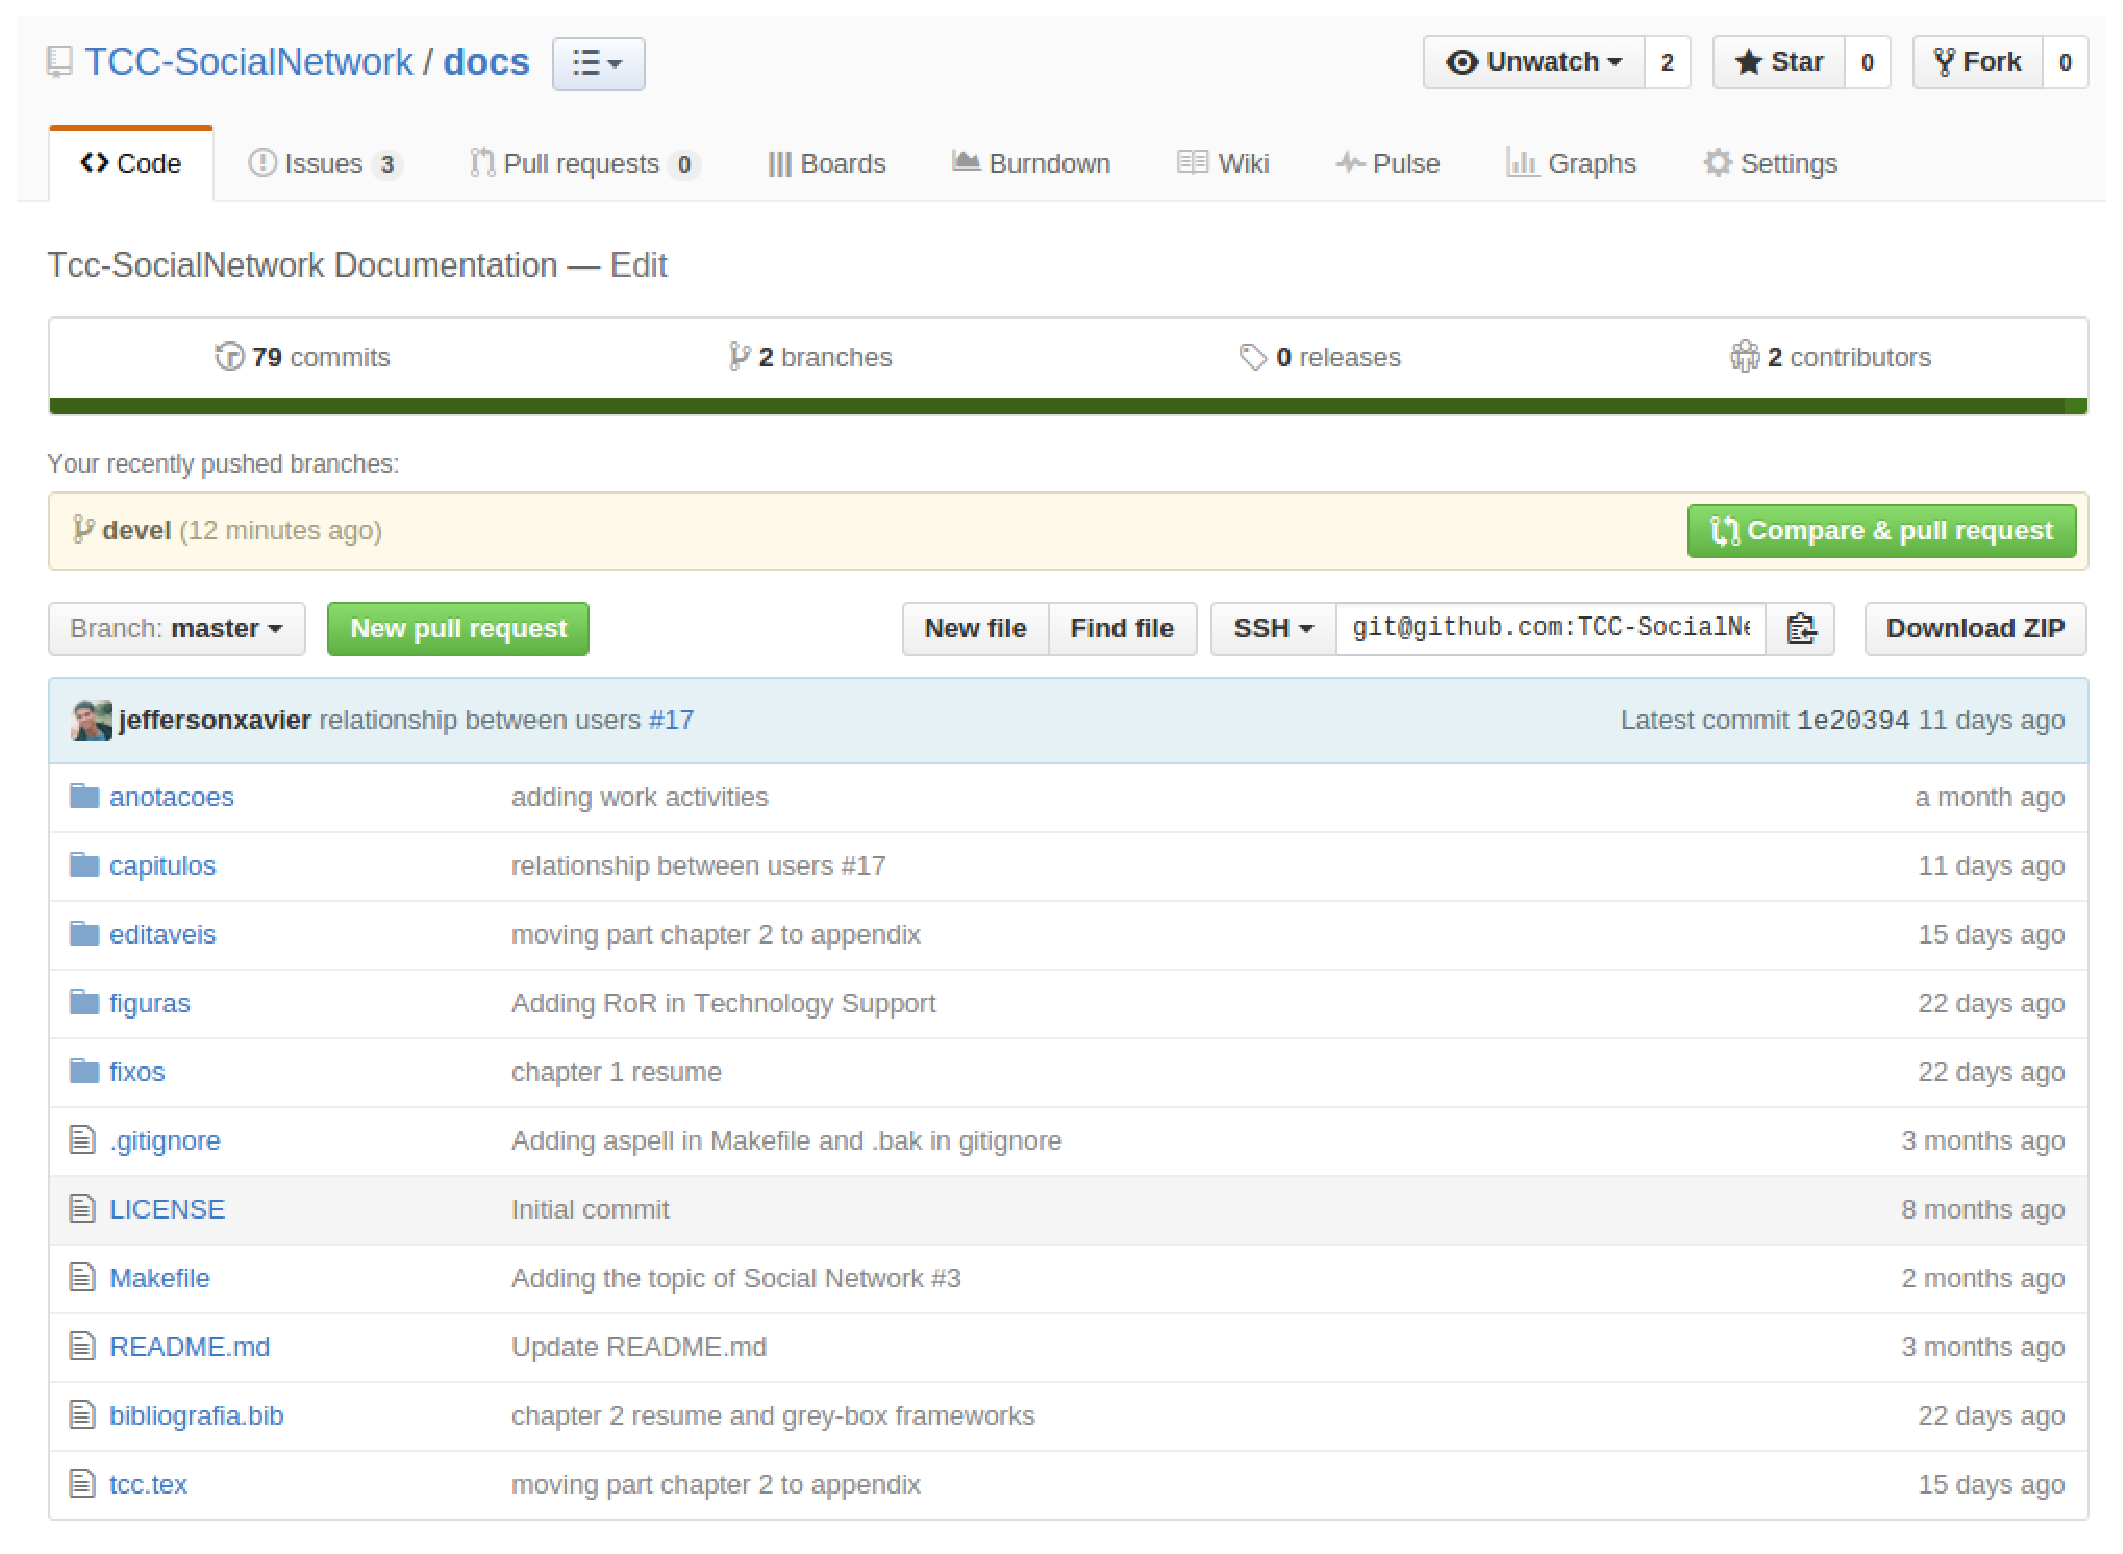
\includegraphics[scale=0.35]{figuras/capitulo3/github.eps}
	\caption{Logo do GitHub}
	\label{github}
\end{figure}

\subsection{ZenHub}

O ZenHub\footnote{\url{https://www.zenhub.io/}}, trata-se de uma extensão para o Chrome para o GitHub, que visa a facilidade as equipes de engenharia a acompanhar o andamento das tarefas de uma forma visual, mostrando-as em um quadro com divisões para cada fase. Com isso pode-se facilmente mover as \textit{issues} entre as fases e acompanhar o andamento do projeto. Outra vantagem em se usar o ZenHub para gerenciar os projetos, é que a sua API pode gerar relatórios, inclusive um \textit{burndown}. O que elimina a necessidade de ferramentas de terceiros de gerenciamento de projeto, criando um local único de foco.

\begin{figure}[!h]
	\centering
	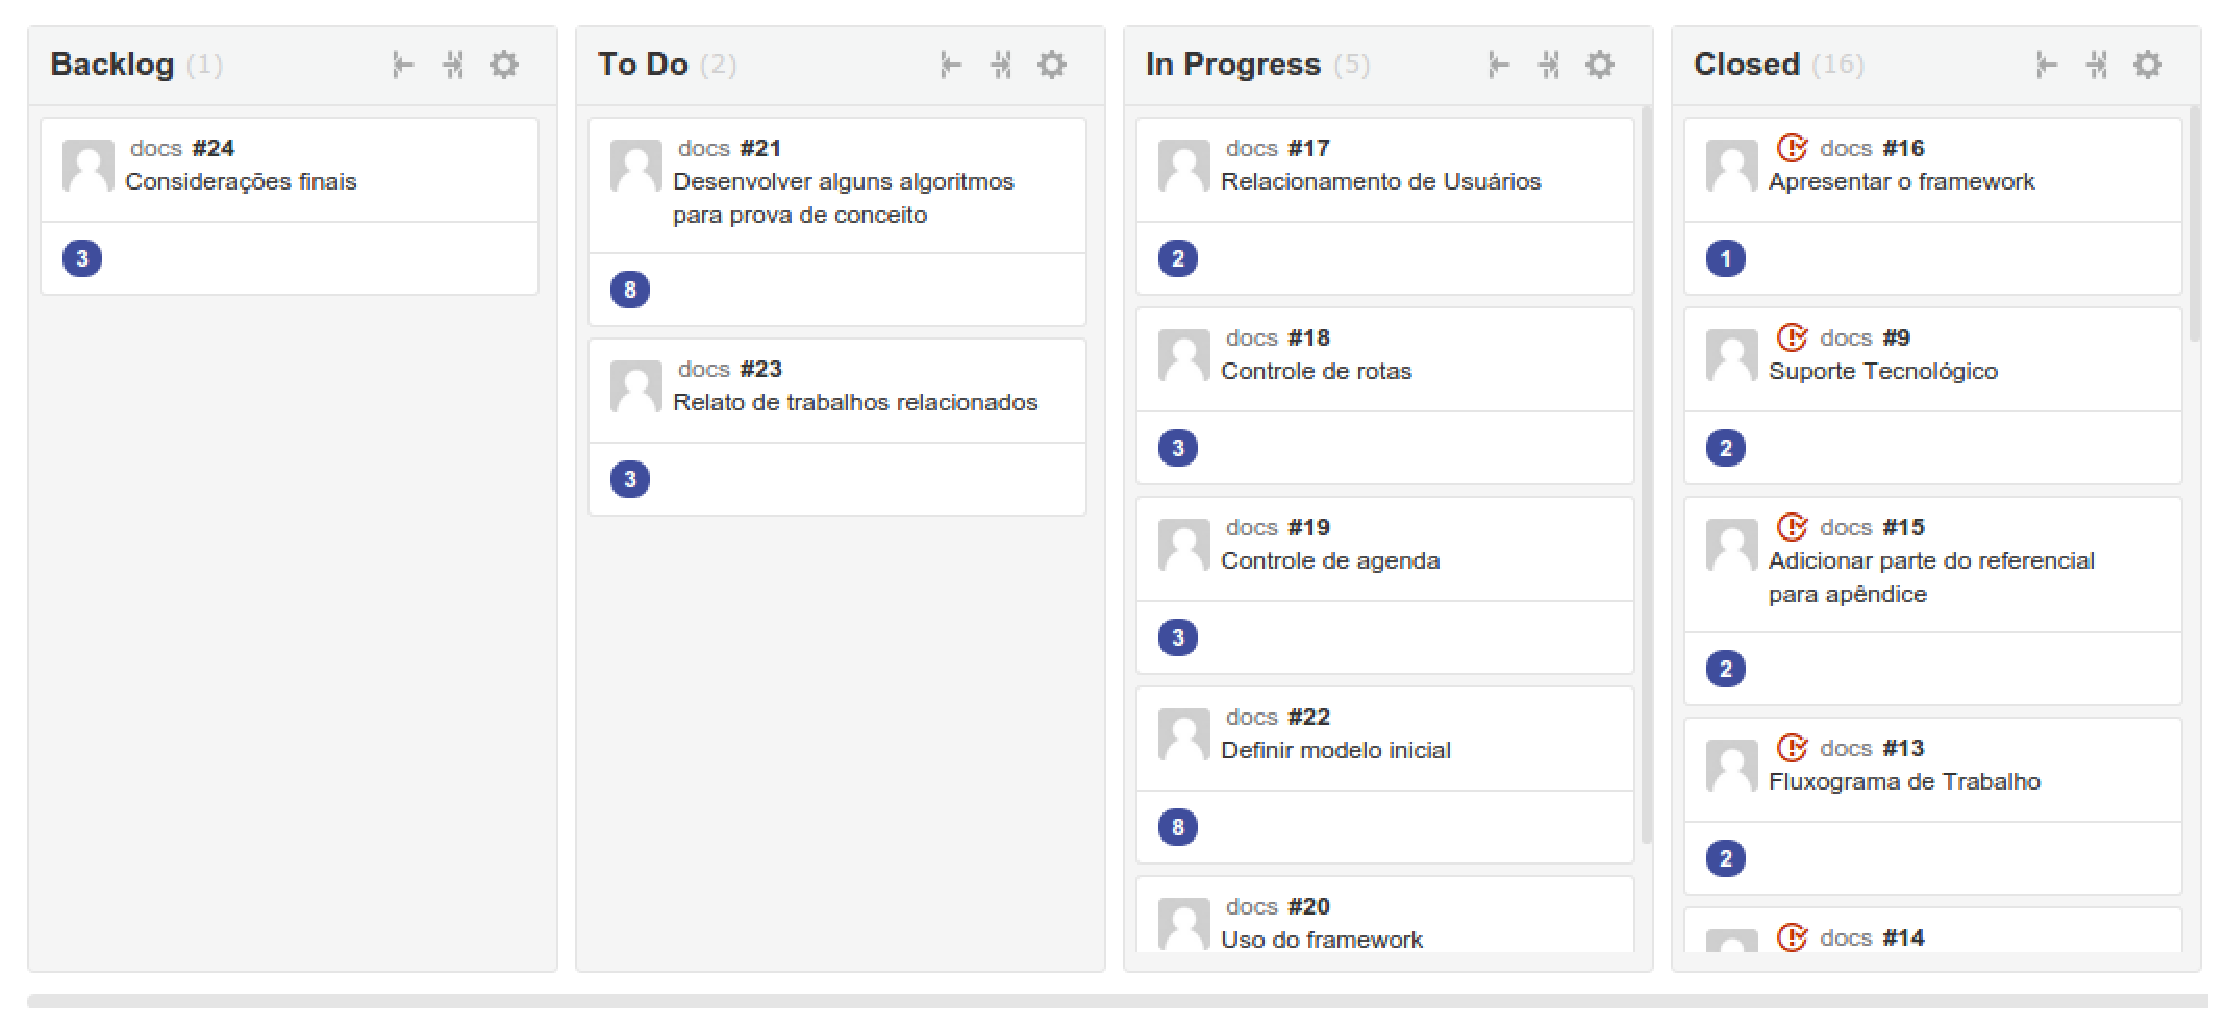
\includegraphics[scale=0.3]{figuras/capitulo3/zenhub.eps}
	\caption{Logo do ZenHub}
	\label{zenhub}
\end{figure}

\subsection{LaTeX}

O \LaTeX\footnote{\url{https://www.latex-project.org}}, é um pacote de macros ou marcações para o processador de textos \TeX. É utilizado amplamente pela comunidade científica devido à sua grande qualidade tipográfica e por torna mais fácil e rápida a produção de documentos em \TeX. O \LaTeX, foi desenvolvido por Leslie Lamport a partir do \TeX, criado por Donald Knuth, e ambos são de código aberto.

O seu objetivo, é que o autor se distancie da apresentação visual do trabalho, e assim, concentrar-se no seu conteúdo. Para isto, ele possui formas de se lidar facilmente com estruturas. Com por exemplo, bibliografias, citações, formatos de páginas e referências. O \LaTeX, não é algo imutável, e como tal, suporta várias maneiras de estilizar e formatar os documentos.

\begin{figure}[!h]
	\centering
	
\includegraphics[scale=0.3]{figuras/capitulo3/latex.eps}
	\caption{Logo do \LaTeX}
	\label{latex}
\end{figure}

\subsection{Sublime Text 3}

Inicialmente pensado pare ser uma extensão do Vim, o Sublime Text\footnote{\url{http://www.sublimetext.com/}} é um editor de texto multiplataforma, escrito em linguagem C++. Com o Sublime é possível automatizar várias tarefas a partir de recursos como, por exemplo, macros, recursos de auto-completar, repetição de ações e construção automática.

Outros recursos como, dividir a tela em várias janelas, auto \textit{save}, navegação entre páginas por meio de abas e suporte a várias linguagens, por exemplo, C, C++, C\#, CSS, HTML, Java, \LaTeX, PHP, Ruby, SQL, XML, JavaScript e Groovy. Fazem do Sublime uma ferramenta poderosa para os programadores.

\begin{figure}[!h]
	\centering
	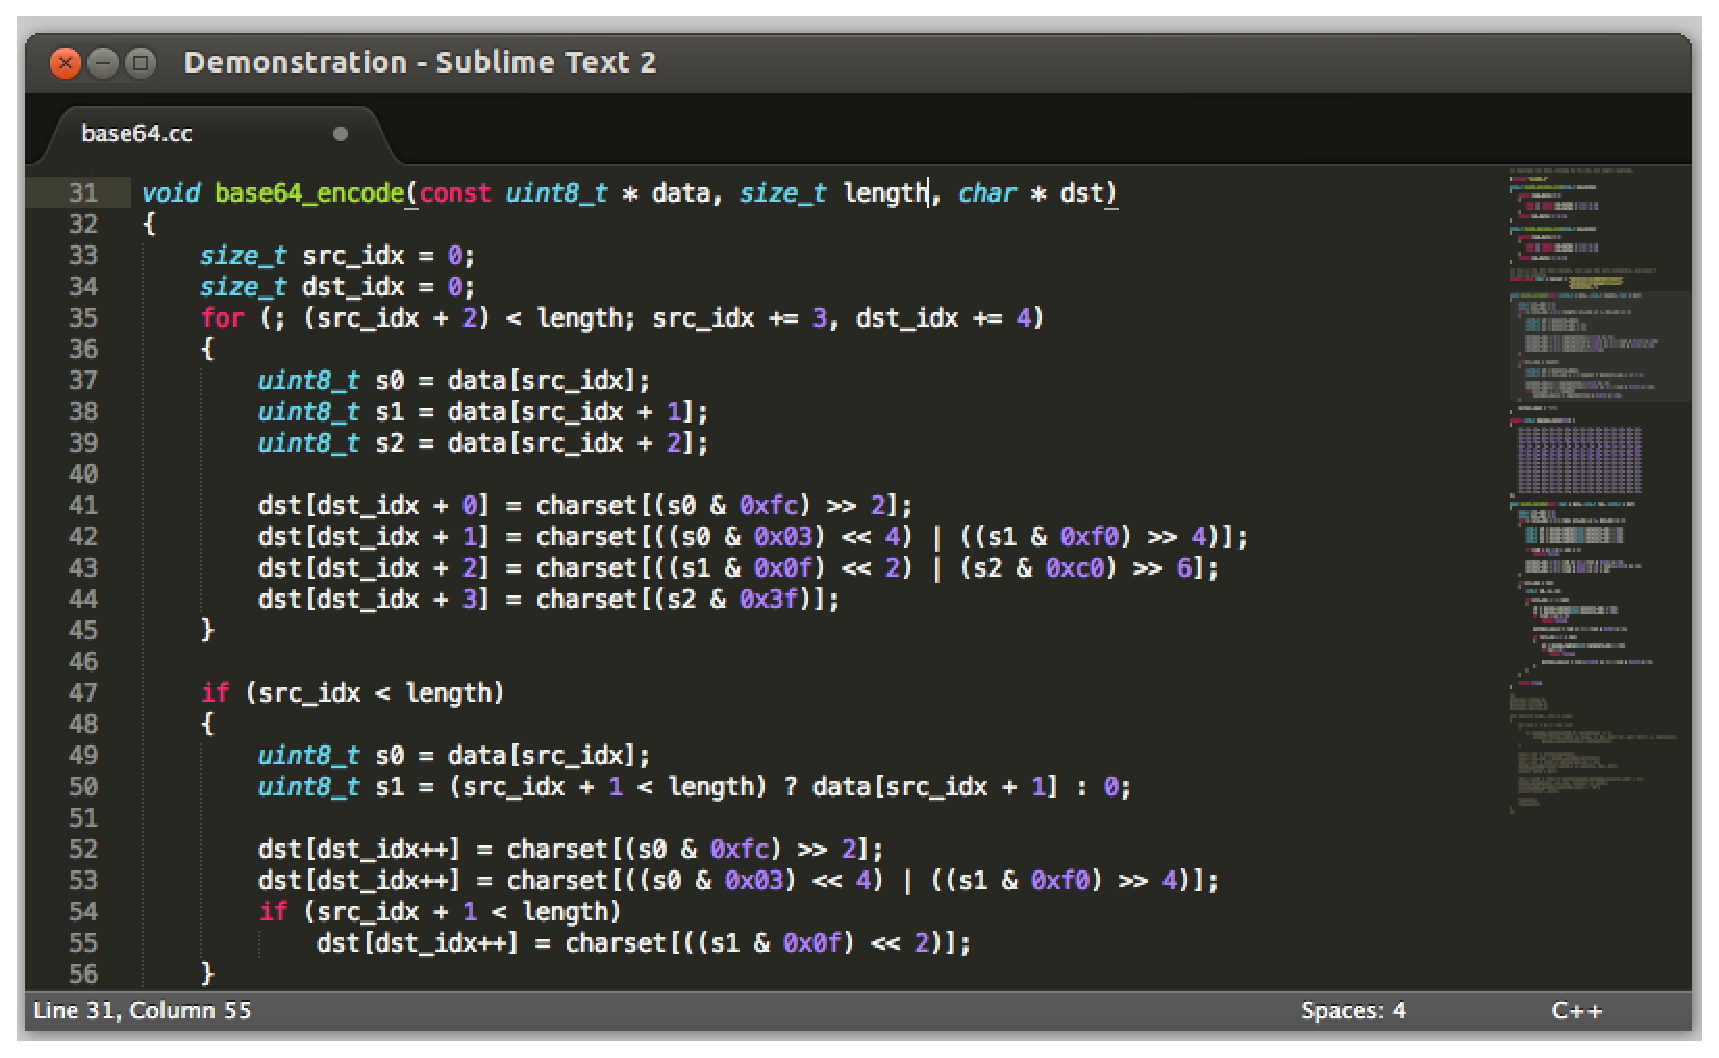
\includegraphics[scale=0.35]{figuras/capitulo3/sublime.eps}
	\caption{Logo do Sublime}
	\label{sublime}
\end{figure}

\subsection{Bizagi Modeler}

Bizagi\footnote{\url{http://www.bizagi.com}} é uma ferramenta para modelar de processos. Esta abrange tanto o mapeamento de processos de trabalho quanto a automação de processos a partir do mapeamento, permitindo que os usuários possam desenhar, documentar e compartilhar seus processos de trabalho usando a notação BPMN (\textit{Business Process Management Notation}). Um diferencial do Bizagi, é a possibilidade de realizar tarefas em conjunto, utilizando um ambiente virtual.

\begin{figure}[!h]
	\centering
	
\includegraphics[scale=0.4]{figuras/capitulo3/bizagi.eps}
	\caption{Logo do Bizagi Modeler}
	\label{bizagi}
\end{figure}

\subsection{Ubuntu}

Ubuntu\footnote{\url{http://www.ubuntu.com/}} é uma palavra de origem africana que significa: ``Humanidade para os outros'' ou ainda ``Sou o que sou pelo que nós somos''. A distribuição Ubuntu traz o espírito desta palavra para o mundo do software livre. Baseado em Linux e criado a partir do Debian. O Ubuntu é patrocinado pela Canonical Ltda., e é licenciado pela licença GPL (\textit{General License Public}).

\begin{figure}[!h]
	\centering
	
\includegraphics[scale=0.4]{figuras/capitulo3/ubuntu.eps}
	\caption{Logo do Ubuntu}
	\label{ubuntu}
\end{figure}

\subsection{Ruby on Rails}

Ruby on Rails \footnote{\url{http://guides.rubyonrails.org/}} é um framework de desenvolvimento de aplicações web escrito na linguagem Ruby. Ele é projetado para tornar a programação de aplicações web mais fácil. A filosofia Rails inclui dois grandes princípios orientadores:

\begin{itemize}
	\item \textbf{DRY:} \textit{Don't Repeat Yourself}, ou não repita a si mesmo, é um princípio de desenvolvimento de software que afirma que ``Cada pedaço de conhecimento deve ter uma única representação inequívoca, e autoritária dentro de um sistema''.

	\item \textbf{Convenção sobre configuração:} É um modelo onde o desenvolvedor precisa de definir apenas aspectos não convencionais da aplicação. Os aspectos convencionais são pré-estabelecidos. Evitando assim o uso maçante de arquivos de configuração.
\end{itemize}

\begin{figure}[!h]
	\centering
	
\includegraphics[scale=0.1]{figuras/capitulo3/ruby_on_rails.eps}
	\caption{Logo do Ruby on Rails}
	\label{ruby_on_rails}
\end{figure}

\section{Resumo do Capítulo}

Este capítulo descreveu o uso das principais ferramentas que serão utilizadas no decorrer deste trabalho. Tais ferramentas visam auxiliar o desenvolvimento do trabalho, tanto na sua documentação, quanto no planejamento e implementação.

No próximo capítulo serão apresentados as metodoligias de pesquisa e desenvolvimento que serão utilizadas no presente deste trabalho.
